\subsection{Saturated Catalyst Model Parameter Estimation}

The linear programming problem is solved using a quadratic polynomial approximation for $\pmb \phi \pmb \theta_{\Gamma scr}$. Both, $k_{scr/asc}$ and $\Gamma$ are assumed to be monotonic functions of temperature but in opposing directions. Thus, just a linear model for the product will not capture the change in monotonic of the product that happens at a particular temperature. After a systematic analysis of various polynomial orders and temperature partitions, a quadratic model with two partitions was found to be the best approximation with minimum prediction error. The parameter estimates of the saturated model are tabulated below.

\begin{table}[H]
        \centering
        \caption{Parameter estimates of the Saturated Catalyst Model of SCR-ASC system}
        \begin{tabular}{l l c c c c}
                \hline \hline
                Age & Test & Temp. Zone &
                $\pmb \theta_{\Gamma scr}[2]$ &
                $\pmb \theta_{\Gamma scr}[1]$ &
                $\pmb \theta_{\Gamma scr}[0]$ \\ \hline \hline
                % ============================================
                Degreened & RMC & high & -0.06 & 1.43 & 31.19 \\
                % =============================================
                Aged & RMC & high & -0.07 & 1.77 & 27.82\\      \hline
                % =============================================
                Degreened & hot-FTP & high & -0.49 & 2.94 & 40.94 \\
                % =============================================
                Aged & hot-FTP & high & -0.54 & 3.40 & 39.59 \\         \hline
                % =============================================
                Degreened & cold-FTP & high & -0.19 & 0.97 & 40.69 \\
                % =============================================
                Aged & cold-FTP & high & -0.28 & 1.82 & 38.97\\         \hline
                % =============================================
                Degreened & cold-FTP & low & 0.26 &  5.97 & 45.00 \\
                % =============================================
                Aged & cold-FTP & low & 0.39 & 8.25 & 50.63 \\
                % =============================================
                \hline \hline
                % =============================================
        \end{tabular}

        $\pmb \theta_{\Gamma scr} [i]$ is the coefficient of $T^i$ in the polynomial.
\end{table}

The parameter values are directionally different for aged and degreened catalyst. Their variance would provide better discernability of the catalyst's aging based on these parameter values.

We have the plots of the response of the saturated system to the inputs from the data as follows.

\begin{figure}[H]
        \begin{minipage}{0.49\textwidth}
                \begin{figure}[H]
                        \centering
                        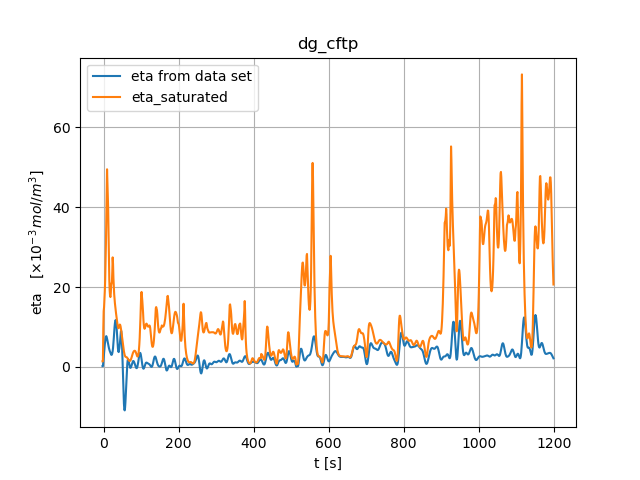
\includegraphics[width=\textwidth]{\froot/figs/14_figs/bounded_eta_plots/eta_bounds_dg_cftp.png}
                \end{figure}
        \end{minipage}
        \begin{minipage}{0.49\textwidth}
                \begin{figure}[H]
                        \centering
                        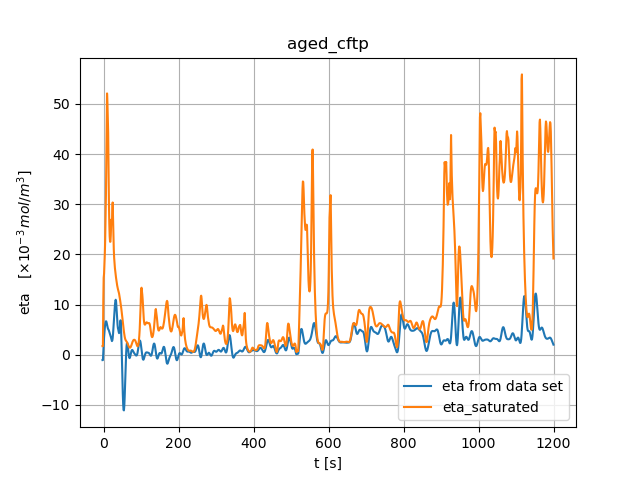
\includegraphics[width=\textwidth]{\froot/figs/14_figs/bounded_eta_plots/eta_bounds_aged_cftp.png}
                \end{figure}
        \end{minipage}
        \caption{Saturated system response for cold FTP data}
\end{figure}

\begin{figure}[H]
        \begin{minipage}{0.49\textwidth}
                \begin{figure}[H]
                        \centering
                        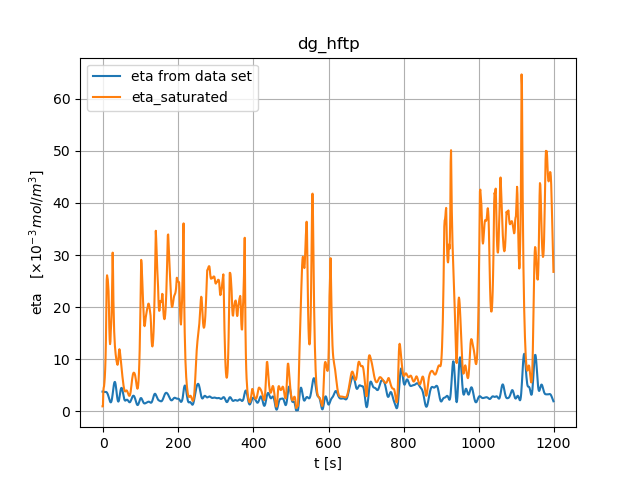
\includegraphics[width=\textwidth]{\froot/figs/14_figs/bounded_eta_plots/eta_bounds_dg_hftp.png}
                \end{figure}
        \end{minipage}
        \begin{minipage}{0.49\textwidth}
                \begin{figure}[H]
                        \centering
                        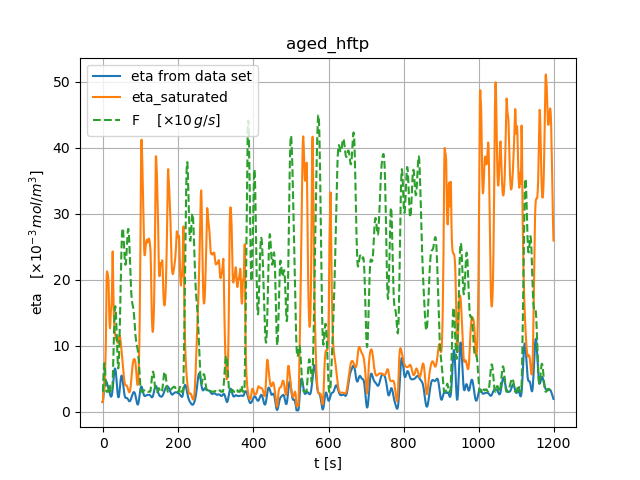
\includegraphics[width=\textwidth]{\froot/figs/14_figs/bounded_eta_plots/eta_bounds_aged_hftp.png}
                \end{figure}
        \end{minipage}
        \caption{Saturated system response for hot FTP data}
\end{figure}

\begin{figure}[H]
        \begin{minipage}{0.49\textwidth}
                \begin{figure}[H]
                        \centering
                        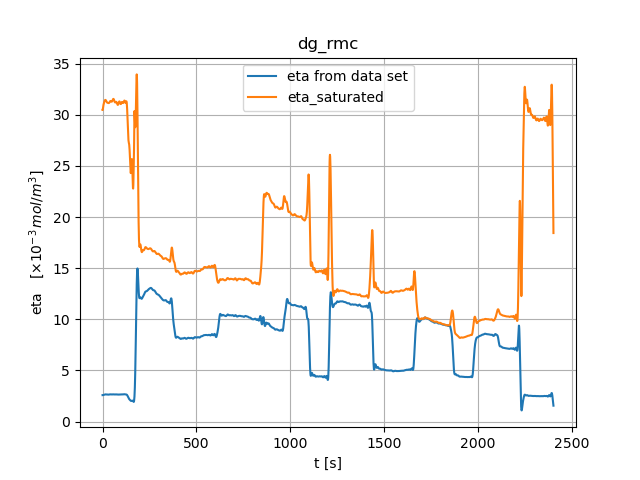
\includegraphics[width=\textwidth]{\froot/figs/14_figs/bounded_eta_plots/eta_bounds_dg_rmc.png}
                \end{figure}
        \end{minipage}
        \begin{minipage}{0.49\textwidth}
                \begin{figure}[H]
                        \centering
                        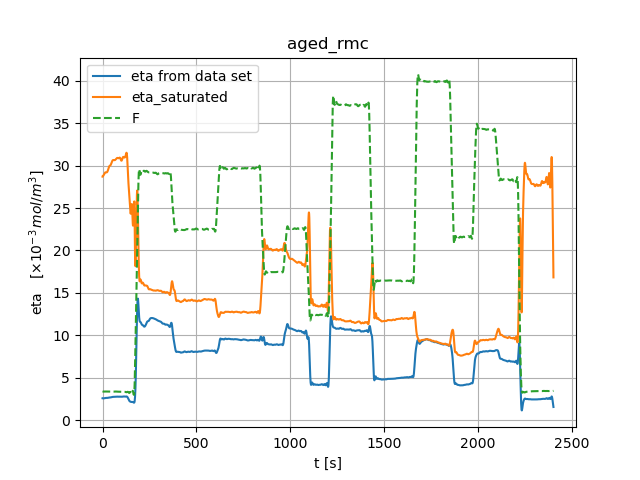
\includegraphics[width=\textwidth]{\froot/figs/14_figs/bounded_eta_plots/eta_bounds_aged_rmc.png}
                \end{figure}
        \end{minipage}
        \caption{Saturated system response for RMC data}
\end{figure}


One observation of note that is consistent with intuition is that the maximum $NO_x$ reduction that is plotted above is
inversely related to the flow-rate of the system. When there is low flow rate, the residence time is high and there is
more time for the $NO_x$ to be reduced at the same reaction rate resulting in higher $NO_x$ reduction.

When this quantity is normalized w.r.t the flow-rate and inlet concentration, we end up with a quantity that is purely a function of temperature  and aging of the catalyst. This is verified in the next section.
